\chapter{Legendre Polinomları}

\section{Giriş}

\medskip
\noindent
\textbf{Bölümün Kapsamı ve Yol Haritası.}
Bu bölümde sırasıyla:
(i) Legendre diferansiyel denklemi ve $P_n(x)$ ailesinin tanımı,
(ii) ortogonallik ve seri açılım katsayılarının projeksiyon mantığıyla elde edilmesi,
(iii) potansiyel teorisi bağlamında sferik harmoniklere geçiş ve fiziksel yorumlar
düzenli bir çerçevede sunulacaktır.


% ============== Tarihçesi ve Motivasyonu ==============
\newpage
\section{Tarihçesi ve Motivasyonu}

Legendre polinomları, matematikteki en temel \textbf{ortogonal polinom aileleri}nden biridir. Bugün yalnızca çekim alanı problemlerinde değil; potansiyel teorisi, elektrostatik,
manyetostatik, ısı iletimi/difüzyon, dalga yayılımı, kuantum mekaniği (özellikle açısal momentum ve küresel simetri),
sayısal analiz (Gauss--Legendre integrasyonu) ve PDE çözümleri (değişkenlerin ayrılması) gibi çok geniş bir alanda karşımıza çıkar.

\medskip
Bu çeşitliliğin ortak nedeni: küresel veya eksenel simetri içeren sistemlerde açısal bağımlılığı düzenli, kararlı ve sistematik biçimde temsil eden doğal baz fonksiyonları olmalarıdır.

\medskip
Yerçekimi ve yörünge mekaniği bağlamında, gerçek gökcisimlerinin (Dünya dâhil) mükemmel küre olmaması nedeniyle ortaya çıkan şekil bozuklukları ve kütle dağılımındaki düzensizlikler, küçük görünse bile hassas yörünge hesaplarında birikimli etkiler üretir. Bu nedenle temel soru şudur:

\begin{quote}
Küresel olmayan bir kütle dağılımının uzayda oluşturduğu çekim potansiyeli,
yeterli doğrulukta ve sistematik biçimde nasıl ifade edilir?
\end{quote}

Pratik yaklaşım, potansiyeli tek adımda kapalı bir integral formunda ifade etmek yerine, onu \textbf{düzenli bir seri açılımı}yla bileşenlerine ayırmaktır. Bu açılımın açısal kısmında Legendre polinomlarının belirmesi tesadüf değildir: uygun koordinatlarda problem ayrıştırıldığında açısal bağımlılık, tam olarak bu polinomların çözdüğü diferansiyel denkleme indirgenir.
Aşağıda bu ihtiyacın tarihsel olarak nasıl olgunlaştığı özetlenmiştir.

% -------------- Newton ve Küre Modeli ------------
\paragraph{1. Newton ve Küre Modeli (1687):}
Isaac Newton, \emph{Principia} (1687) adlı eserinde homojen bir kürenin, dış uzaydaki çekim etkisinin, tüm kütlesi merkezde toplanmış tek bir noktasal kütleninkiyle aynı olduğunu gösterdi. Bu yüzden küre dışındaki bir noktada yerçekimi potansiyeli,
merkezi çekim formunda

\begin{equation}
U(\mathbf{r})=-\frac{\mu}{\lVert \mathbf{r}\rVert},
\qquad \mu \equiv GM.
\label{eq:pointmass_potential}
\end{equation}

şeklinde yazılabilir. Bu idealizasyon yerçekimi problemlerine güçlü ve sade bir başlangıç sunsa da, Dünya’nın dönmeye bağlı basıklığı ve kütle dağılımındaki düzensizlikler nedeniyle
gerçek alan bu basit modelden düzenli olarak sapar. Dolayısıyla daha yüksek doğruluk için merkezi potansiyelin üzerine  \textbf{küresel olmayan} (\emph{asferik}) düzeltmeler eklemek gerekir.

% ------------- Dünyanın Şekli Üzerine Tartışmalar ----------
\paragraph{2. Dünya’nın Şekli Üzerine Tartışmalar (1700'ler)}
Dünya’nın dönmesi, merkezkaç etkisi nedeniyle yaklaşık olarak \textbf{kutuplardan basık} (\emph{oblate}) bir denge şekline işaret eder. Nitekim Newton (ve aynı dönemde Huygens) dönmenin Dünya’yı kutuplardan basıklaştıracağını öngörürken,
Cassini ailesinin Fransa’daki erken meridyen yayı ölçümlerine dayanan yorumu bir süre Dünya’nın \textbf{kutuplardan uzun} (\emph{prolate}) olabileceği yönünde bir karşı görüşü beslemiştir.
Ancak erken dönem ölçümlerin sınırlı doğruluğu ve veri yorumundaki belirsizlikler, bu tür zıt sonuçların aynı anda savunulabilmesine imkân vermiştir. 

% -------------- Jeodezik Seferler ---------------
\paragraph{3. Jeodezik Seferler ve Sonucun Netleşmesi (1730'lar)}
18.\ yüzyılın ilk yarısındaki jeodezik ölçüm seferleri,
Dünya’nın \textbf{kutuplardan basık} olduğu sonucunu güçlü biçimde desteklemiştir. Böylece küre modeli “iyi bir ilk yaklaşım” olarak kalmış, ancak küresel sapmaların potansiyele sistematik biçimde eklenmesi ihtiyacı netleşmiştir.

% ---------------- Maclaurin ve Clairaut ------------
\paragraph{4. Maclaurin ve Clairaut: Dönen Cisimler ve Sferoid Modelleri (1740'lar)} Maclaurin dönen akışkan kütlelerin denge şekillerini inceleyerek \textbf{Maclaurin sferoidi} çerçevesini geliştirmiş, Clairaut ise basıklık ile yerçekiminin enleme bağlı değişimi arasındaki ilişkiyi teorik olarak temellendirmiştir.
Bu çalışmalar, \textbf{küre dışı} etkilerin nicel modellemenin ayrılmaz parçası olduğunu göstermiştir.


% ------------- Legendre Polinomları  ----------------
\paragraph{5. Legendre: Seri Açılım ve $P_n$’lerin Ortaya Çıkışı (1782)}
18.\ yüzyılın sonlarına gelindiğinde, Dünya’nın küresel olmayan şeklinin yerçekimi alanına etkisi daha sistematik
biçimde ele alınmaya başlandı. Bu bağlamda Legendre’nin 1782’de sferoitlerin çekimi üzerine yaptığı çalışmalar,
potansiyel hesabındaki temel güçlüğü netleştirdi: kütle elemanları ile gözlem noktası arasındaki
\(\lvert \mathbf{r}-\mathbf{r}_Q\rvert^{-1}\) bağımlılığını açısal değişkenlere göre düzenli ve hesaplanabilir bir biçimde ayrıştırmak.
Legendre’nin çalışmaları, bu geometrik bağımlılığın bir polinom ailesi üzerinden seri hâlinde ifade edilebileceğini ortaya koymuş
ve böylece potansiyelin derece derece ayrıştırılmasına dayanan yaklaşımın
(ileride küresel harmonik açılımın matematiksel omurgasını oluşturacak olan)
temelini atmıştır. Bu fikir, Legendre polinomlarının üreteç fonksiyonunda açıkça görülür:

\begin{equation}
\frac{1}{\sqrt{1-2\frac{r_Q}{r}\,x+\left(\frac{r_Q}{r}\right)^2}}
=
\sum_{n=0}^{\infty}P_n[x]\left(\frac{r_Q}{r}\right)^n,
\qquad r=\lVert\mathbf{r}\rVert,\ \ r_Q=\lVert\mathbf{r}_Q\rVert.
\label{eq:legendre_generating_function}
\end{equation}





Bu sayede tek bir zor integral yerine, terim terim ilerleyen; hem hesaplamaya elverişli hem de fiziksel yoruma açık bir temsil elde edilir. Bu bakış açısı, yerçekimi potansiyelini merkezi terim ve asferik düzeltmelerin toplamı olarak yazmayı mümkün kılmıştır:

\[
U = U_0 + U_1 + U_2 + \cdots + U_n.
\]


% --------------- Laplace ve Sferik Harmonikler ----------
\paragraph{6. Laplace: Ayrılabilirlik ve Sferik Harmonikler (1799--1820'ler)}
Legendre’nin seri açılımı, çekim problemlerinde ``açısal bağımlılığı'' yönetilebilir hâle getirmişti.
Laplace ise 1799’dan itibaren bu fikri daha genel bir çerçeveye oturttu:
kaynak bulunmayan dış uzayda yerçekimi potansiyelinin Laplace denklemini sağladığını gösterdi ve
bu denklemin küresel koordinatlarda doğal olarak \textbf{derece derece }çözümlere ayrıldığını ortaya koydu.
Bu çözüm ailesinin açısal parçası Legendre denklemiyle belirlenirken, azimutal bağımlılık da eklendiğinde ilişkili Legendre fonksiyonları ve sferik harmonikler ortaya çıkar.
Bugün gravite modellerinde gördüğümüz $C_{\ell,m}$ ve $S_{\ell,m}$ katsayıları, tam olarak bu sferik harmonik çözüm ailesinin genliklerini (ağırlıklarını) temsil eder.



% ----------------- Kuramsal Çerçeve -------------
\paragraph{7. 19.\ yüzyıl: Kuramsal Çerçeve ve Hesap Yöntemleri}
19.\ yüzyılda Legendre polinomları artık yalnızca ``özel bir seri açılımı'' olmaktan çıkıp,
hem kuramsal hem de hesaplamalı araçlar açısından olgun bir çerçeveye kavuştu.
Rodrigues formülü ve rekürans bağıntıları, $P_\ell$’lerin düzenli ve verimli biçimde üretilmesini mümkün kılarken,
Sturm--Liouville kuramı bu fonksiyon ailesinin neden ortogonal olduğunu ve hangi norm yapısı altında çalıştığını
özdeğer problemi bakışıyla sistematikleştirdi.
Aynı dönemde Gauss’un çalışmaları, $P_\ell$ köklerini düğüm noktaları olarak kullanan
\textbf{Gauss--Legendre integrasyonu}nu öne çıkardı; bu yöntem özellikle pürüzsüz integraller için
yüksek doğrulukla sayısal hesap yapmanın standart yollarından biri hâline geldi.
Böylece Legendre polinomları, bir yandan analitik modellemede ``derece derece'' temsil fikrini taşırken,
diğer yandan pratik hesaplarda güvenilir ve tekrarlanabilir bir sayısal altyapı sağlamış oldu.


% ============ Legendre Polinom Katsayılarının Hesaplanması =======
\newpage
\section{Legendre Polinomlarının Ortaya Çıkışı}

Legendre polinomlarının ortaya çıkışı, yukarıda da bahsettiğimiz gibi,
Legendre’in 1780’lerin başında gezegenlerin (yani küresel olmayan cisimlerin)
kütle çekim potansiyelini incelemesiyle başlar.
Küre gibi mükemmel simetrili bir cismin dış uzaydaki potansiyeli
Newton teorisinden zaten bellidir:
\begin{equation}
U(r)= -\frac{\mu}{r}.
\end{equation}
Ancak gezegen küresel değilse, artık tüm kütleyi merkezde toplanmış gibi düşünemeyiz.
Kütle uzaya yayıldığı için potansiyeli bulmak adına
cismin tamamı üzerinden sürekli bir integral almak gerekir.
Bu durumda gözlem noktası $P$ için potansiyel
\begin{equation}
U( r)
=
-G\iiint_{\text{Cisim}}\frac{dm}{\rho_Q}
\label{eq:U_integral}
\end{equation}
şeklinde yazılır.
Burada $\rho_Q=\|\mathbf r-\mathbf r_Q\|$,
cismin içindeki kütle elemanı $m_Q$ ile gözlem noktası $P$ arasındaki uzaklıktır.

\begin{figure}[h]
  \centering
  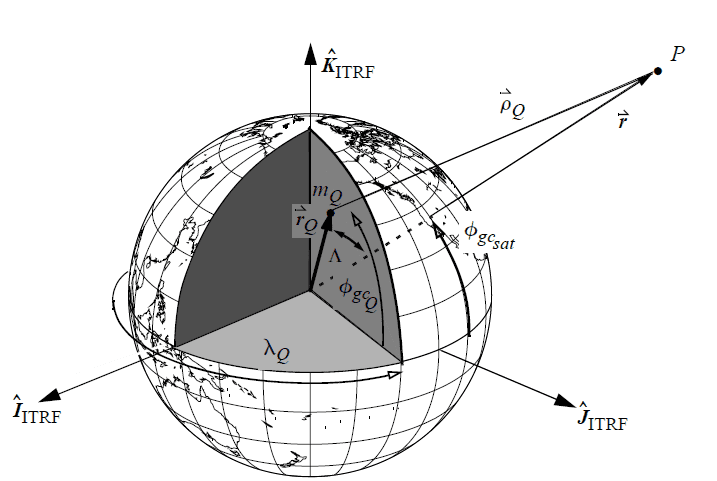
\includegraphics[width=0.75\linewidth]{Resimler/Earth Gravitational Potential.png}
  \caption{Dünya içindeki bir kütle elemanı $m_Q$ (konumu $\mathbf r_Q$) ile dış uzaydaki gözlem noktası $P$ (konumu $\mathbf r$) arasındaki geometri.}
  \label{fig:earth_potential_geometry}
\end{figure}

Şekil~\ref{fig:earth_potential_geometry}’de görülen $\Lambda$ açısı,
$\mathbf r$ ile $\mathbf r_Q$ doğrultuları arasındaki açıdır.
Kosinüs teoremi kullanılarak iki nokta arasındaki uzaklık
\begin{equation}
\rho_Q^{\,2}
=
r^2+r_Q^2-2rr_Q\cos\Lambda
\label{eq:rhoQ_coslaw_here}
\end{equation}
şeklinde elde edilir.
Dış uzaydaki bir gözlem noktası için genellikle $r>r_Q$ olduğundan
\begin{equation}
\alpha=\frac{r_Q}{r}
\qquad (0\le \alpha<1)
\label{eq:alpha_def_here}
\end{equation}
oranı tanımlanır.
Böylece \eqref{eq:rhoQ_coslaw_here} ifadesi
\begin{equation}
\rho_Q
=
r\sqrt{1-2\alpha\cos\Lambda+\alpha^2}
\label{eq:rhoQ_alpha_here}
\end{equation}
biçimine indirgenir ve integrand
\begin{equation}
\frac{1}{\rho_Q}
=
\frac{1}{r}\,
\frac{1}{\sqrt{1-2\alpha\cos\Lambda+\alpha^2}}
\label{eq:inv_rhoQ_factor}
\end{equation}
haline gelir.


Legendre \eqref{eq:inv_rhoQ_factor} ifadesinde hem $r$ hem $r_Q$ (yani $\alpha$), hem de açıya bağlı $\cos\Lambda$ aynı karekökün içinde birbirine karıştığını fark etmişti. Bu şekilde integrali doğrudan almak çoğu zaman çok zor olduğundan doğrudan integral almak yerine ne yapabilirim diye düşündü. Bunun üzerine integraldeki $1/\rho_Q$ ifadesini, $r$ ve $r_Q$ birbirinden ayrılmış şekilde bir seri haline getirip integralini alabileceğini farketti.

\medskip
 $\alpha=r_Q/r<1$ olduğundan \eqref{eq:inv_rhoQ_factor} içindeki
\(\bigl(1-2\alpha\cos\Lambda+\alpha^2\bigr)^{-1/2}\) ifadesini
$\alpha$ cinsinden bir seri olarak açmak mümkündür.
Legendre, Taylor açılımının atası sayılan Newton binom açılımını
bu tür ifadeler üzerinde kullanıp terimleri düzenlediğinde,
$\alpha$ kuvvetlerinin katsayılarının sadece açıya bağlı kaldığını, hatta bunun $\cos\Lambda$ cinsinden bir polinom ailesi oluşturduğunu görür. Bu polinomları sistematik biçimde tanımlamak için de \textbf{}{üretici fonksiyon} (\emph{generating function}) fikrini ortaya koyar.

\medskip
\noindent
\textbf{Newton binom açılımı:}
Dış bölgede $\alpha<1$ olduğundan, şu ifadeyi $\alpha$ cinsinden seri açabiliriz:
\begin{equation}
\frac{1}{\sqrt{1-2\alpha\cos\Lambda+\alpha^2}}
=
\left(1+u\right)^{-1/2},
\qquad
u:=\alpha^2-2\alpha\cos\Lambda.
\label{eq:u_def}
\end{equation}
Genelleştirilmiş Newton binom açılımı
\begin{equation}
(1+u)^{-1/2}
=
1-\frac{1}{2}u+\frac{3}{8}u^2-\frac{5}{16}u^3+\mathcal{O}(u^4)
\label{eq:newton_binom_series}
\end{equation}
şeklindedir.
Şimdi $u=\alpha^2-2\alpha\cos\Lambda$ yerine koyup,
$\alpha$ mertebelerine göre terimleri toplayalım.

Önce $u$ ve kuvvetlerini $\alpha$ cinsinden açalım:
\begin{align}
u &= \alpha^2-2\alpha\cos\Lambda,\\[4pt]
u^2 &= (\alpha^2-2\alpha\cos\Lambda)^2
= \alpha^4 -4\alpha^3\cos\Lambda +4\alpha^2\cos^2\Lambda,\\[4pt]
u^3 &= (\alpha^2-2\alpha\cos\Lambda)^3
= \alpha^6 -6\alpha^5\cos\Lambda +12\alpha^4\cos^2\Lambda -8\alpha^3\cos^3\Lambda.
\end{align}

Bunları \eqref{eq:newton_binom_series} içine koyup
$\alpha^3$ mertebesine kadar (yani $\mathcal{O}(\alpha^4)$’e kadar ihmal ederek)
toplayalım.

\paragraph{1) $-\tfrac12 u$ katkısı:}
\begin{equation}
-\frac12 u
=
-\frac12(\alpha^2-2\alpha\cos\Lambda)
=
\alpha\cos\Lambda-\frac12\alpha^2.
\end{equation}

\paragraph{2) $\tfrac{3}{8}u^2$ katkısı:}
$\alpha^3$’e kadar sadece $\alpha^2$ ve $\alpha^3$ terimleri gerekli:
\begin{equation}
\frac{3}{8}u^2
=
\frac{3}{8}\left(4\alpha^2\cos^2\Lambda -4\alpha^3\cos\Lambda + \alpha^4\right)
=
\frac{3}{2}\alpha^2\cos^2\Lambda
-\frac{3}{2}\alpha^3\cos\Lambda
+\mathcal{O}(\alpha^4).
\end{equation}

\paragraph{3) $-\tfrac{5}{16}u^3$ katkısı:}
$\alpha^3$ mertebesine kadar yalnızca $-8\alpha^3\cos^3\Lambda$ terimi önemlidir:
\begin{equation}
-\frac{5}{16}u^3
=
-\frac{5}{16}\left(-8\alpha^3\cos^3\Lambda+\mathcal{O}(\alpha^4)\right)
=
\frac{5}{2}\alpha^3\cos^3\Lambda
+\mathcal{O}(\alpha^4).
\end{equation}

\paragraph{4) Tüm katkıların toplanması.}
Şimdi tüm parçaları bir araya getirirsek:
\begin{align}
\frac{1}{\sqrt{1-2\alpha\cos\Lambda+\alpha^2}}
&=
1
+\left(\alpha\cos\Lambda\right) \nonumber\\
&\quad
+\alpha^2\left(\frac{3}{2}\cos^2\Lambda-\frac{1}{2}\right)\nonumber\\
&\quad
+\alpha^3\left(\frac{5}{2}\cos^3\Lambda-\frac{3}{2}\cos\Lambda\right)
+\mathcal{O}(\alpha^4).
\label{eq:explicit_series_alpha}
\end{align}

Bu sonuç çok önemli bir şeyi açıkça gösterir:
$\alpha$ kuvvetlerinin katsayıları,
sadece $\cos\Lambda$'ya bağlı \textbf{polinomlar}dır.
Gerçekten de
\begin{align}
P_0[\cos\Lambda]&=1,\\
P_1[\cos\Lambda]&=\cos\Lambda,\\
P_2[\cos\Lambda]&=\frac12\left(3\cos^2\Lambda-1\right),\\
P_3[\cos\Lambda]&=\frac12\left(5\cos^3\Lambda-3\cos\Lambda\right),
\end{align}
olduğundan \eqref{eq:explicit_series_alpha} ifadesi,
Legendre polinomlarının ürettiği seriyle birebir örtüşür:
\begin{equation}
\frac{1}{\sqrt{1-2\alpha\cos\Lambda+\alpha^2}}
=
\sum_{n=0}^{\infty}P_n[\cos\Lambda]\,\alpha^n,
\qquad (0\le \alpha<1).
\end{equation}


Denklemde $\cos\Lambda \Rightarrow x, \qquad \alpha \Rightarrow \frac{r_Q}{r}$ yazıldığında \eqref{eq:inv_rhoQ_factor} doğrudan seri açılır:
\begin{equation}
\frac{1}{\rho_Q}
=
\frac{1}{r}
\sum_{n=0}^{\infty}
P_n[\cos\Lambda]\,\alpha^n
=
\frac{1}{r}
\sum_{n=0}^{\infty}
P_n[x]\left(\frac{r_Q}{r}\right)^n,
\qquad (r>r_Q).
\label{eq:1_over_rhoQ_legendre}
\end{equation}
Buradaki $P_n(\cdot)$ polinomları,
bugün \textbf{Legendre polinomları} olarak bildiğimiz polinom ailesidir.

Resimde görüldüğü üzere ilk 6 Legendre polinomu,
$[-1,1]$ aralığında çizdirilmiştir.

\begin{figure}[h]
    \centering
    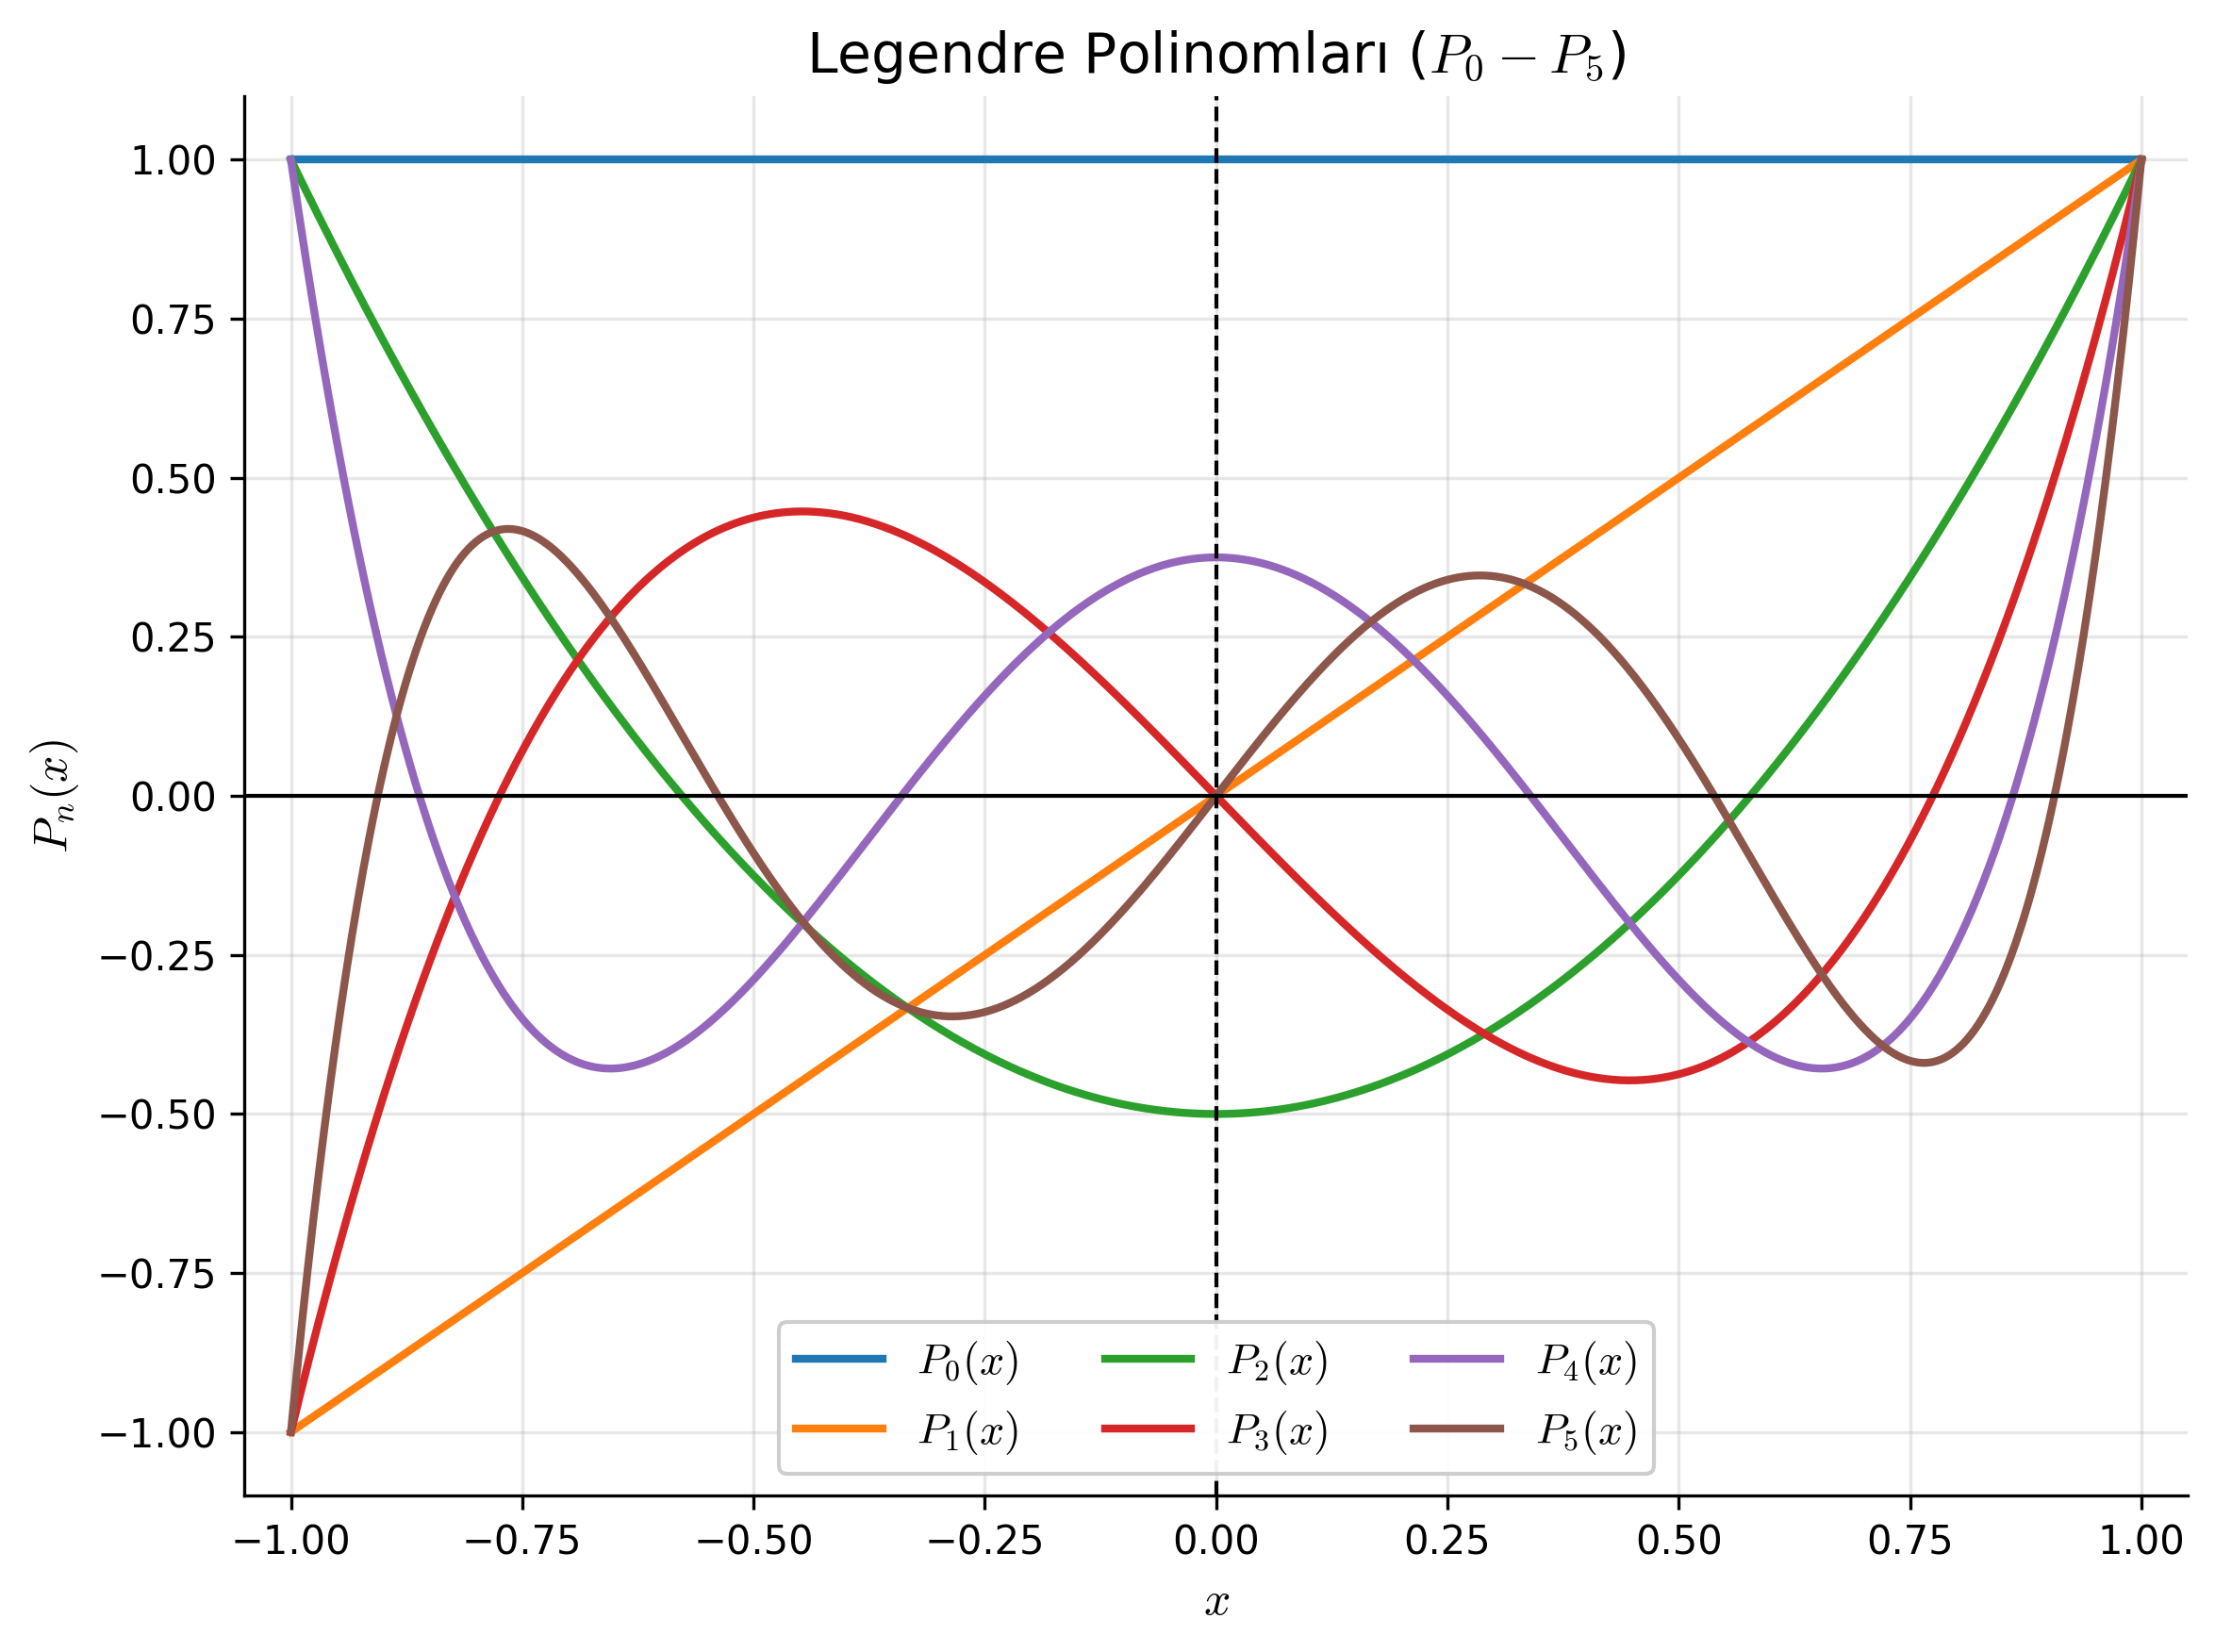
\includegraphics[width=0.6\linewidth]{Resimler/Poly First 6.png}
    \caption{$[-1,1]$ aralığında ilk 6 Legendre polinomu ($P_0$--$P_5$).}
    \label{fig:Legendre_poly_first6}
\end{figure}



\newpage
\subsection{Legendre'den Sonra}

Legendre’in potansiyel probleminden hareketle tanımladığı bu polinomlar, zamanla matematiksel açıdan da büyük önem kazandı.
Özellikle 19. yüzyılda, Legendre polinomlarının farklı yollarla yeniden üretilebildiği ve bu polinomlar için pratik kapalı ifadeler yazılabildiği gösterildi. Bunların en kullanışlı örneklerinden biri, \textbf{Olinde Rodrigues}’in 1816’da verdiği üretim formülüdür. Legendre’in yaklaşımından birkaç on yıl sonra ortaya çıkan bu sonuç, $P_n(x)$ polinomlarını doğrudan üretmek için güçlü bir kısa yol sağlar.

% ------------------------------------------------------------
\subsubsection{Rodrigues Formülü}

Legendre polinomlarının en bilinen kapalı üretim ifadelerinden biri Rodrigues formülüdür:
\begin{equation}
P_n(x)=\frac{1}{2^n n!}\frac{d^n}{dx^n}\Big[(x^2-1)^n\Big].
\label{eq:Rodrigues}
\end{equation}

Bu formül iki noktayı aynı anda netleştirir:
(i) $P_n(x)$ gerçekten bir polinomdur,
(ii) derecesi de tam olarak $n$’dir.
Çünkü $(x^2-1)^n$ ifadesi binom açılımı ile sonlu sayıda terime ayrılır:
\[
(x^2-1)^n
= \sum_{k=0}^{n}\binom{n}{k}(x^2)^{\,n-k}(-1)^k
= \sum_{k=0}^{n}\binom{n}{k}(-1)^k x^{2(n-k)}.
\]
Bu polinomun en yüksek derecesi $2n$’dir.
$n$ kez türev alındığında derecesi $2n-n=n$ olur ve sonuç yine polinom kalır.
Dolayısıyla $P_n$ notasyonu, polinomun derecesiyle doğrudan uyumludur.

% ------------------------------------------------------------
\subsubsection{Rodrigues ile İlk 10 Legendre Polinomu}

Rodrigues formülü \eqref{eq:Rodrigues} kullanılarak $P_n(x)$ polinomları
tek tek üretilebilir. Aşağıda $n=0$ ile $n=9$ arasındaki ilk 10 Legendre polinomu
tablo halinde verilmiştir.

\begin{table}[h]
\centering
\renewcommand{\arraystretch}{1.5}
\setlength{\tabcolsep}{12pt}
\begin{tabular}{c l c l}
\toprule
\textbf{$n$} & \textbf{$P_n(x)$} & \textbf{$n$} & \textbf{$P_n(x)$} \\
\midrule
0 & $1$
& 5 & $\frac{1}{8}\,(63x^5-70x^3+15x)$ \\[6pt]

1 & $x$
& 6 & $\frac{1}{16}\,(231x^6-315x^4+105x^2-5)$ \\[6pt]

2 & $\frac{1}{2}\,(3x^2-1)$
& 7 & $\frac{1}{16}\,(429x^7-693x^5+315x^3-35x)$ \\[6pt]

3 & $\frac{1}{2}\,(5x^3-3x)$
& 8 & $\frac{1}{128}\,(6435x^8-12012x^6+6930x^4-1260x^2+35)$ \\[8pt]

4 & $\frac{1}{8}\,(35x^4-30x^2+3)$
& 9 & $\frac{1}{128}\,(12155x^9-25740x^7+18018x^5-4620x^3+315x)$ \\
\bottomrule
\end{tabular}
\caption{Rodrigues formülü ile üretilen ilk 10 Legendre polinomu ($P_0$--$P_9$).}
\label{tab:first10_legendre}
\end{table}



% ========== Ek Okuma ve Alternatif Yaklaşımlar ===========
\newpage
\section{Ek Okuma ve Teorik Arkaplan}
\label{subsec:ek_okuma_alternatifler}

Rodrigues formülü, Legendre polinomlarını üretmek için son derece pratik bir araçtır. Ancak bu polinomların nereden çıktığını ve diğer ortogonal polinom aileleriyle nasıl ilişkilendiğini bilmek, özellikle mühendislikte \uline{doğru probleme doğru baz} seçebilmek açısından önemlidir. Bu alt bölümde, Legendre polinomlarının diferansiyel denklem kökeni, cebirsel inşası ve alternatif ortogonal bazlarla ilişkisi özetlenmektedir.

% ------------------------------------------------------------
\subsection{Diferansiyel Denklem Kökeni ve Sturm--Liouville}

Legendre polinomları, küresel simetri içeren problemlerde (özellikle Laplace denklemi)
değişkenlerin ayrılması uygulanınca doğal olarak ortaya çıkan Legendre diferansiyel denkleminin çözümleridir:
\begin{equation}
(1-x^2)\,y''-2x\,y' + n(n+1)\,y = 0.
\label{eq:legendre_de_bg}
\end{equation}
Bu denklem Sturm--Liouville formuna da yazılabilir:
\begin{equation}
\frac{d}{dx}\!\left[(1-x^2)\,y'\right] + n(n+1)\,y = 0,
\qquad x\in[-1,1].
\label{eq:legendre_sl_form}
\end{equation}


Pek çok fiziksel problem (titreşim modları, ısı iletimi, potansiyel problemleri vb.) uygun sınır koşulları altında bir \textbf{özdeğer problemi}ne indirgenir ve bu problemler çoğunlukla

\begin{equation}
\frac{d}{dx}\!\left[p(x)\,y'\right] + \bigl[\lambda\,w(x)-q(x)\bigr]\,y = 0,
\qquad w(x)>0
\label{eq:sl_general}
\end{equation}

şeklinde yazılabilir. Buradaki kritik nokta, çözüm ailesinin doğal olarak bir \textbf{ağırlık fonksiyonu} $w(x)$ ile birlikte gelmesidir.

Sturm--Liouville teorisi gereğince, \eqref{eq:sl_general} biçimindeki bir özdeğer probleminde
farklı özdeğerlere karşılık gelen özfonksiyonlar,
\begin{equation}
\int_{-1}^{1} y_n(x)\,y_m(x)\,w(x)\,dx = 0 \qquad (n\neq m)
\label{eq:sl_ortho_general}
\end{equation}
anlamında \textbf{ağırlıklı} ortogonaldir.

Legendre durumunda \eqref{eq:legendre_sl_form} ile karşılaştırınca
$p(x)=1-x^2$, $q(x)=0$, $\lambda=n(n+1)$ ve en önemlisi $w(x)=1$ elde edilir.
Dolayısıyla ortogonallik, klasik (ağırlıksız) biçime indirgenir:

\begin{equation}
\int_{-1}^{1} P_n(x)\,P_m(x)\,dx = 0 \qquad (n\neq m).
\label{eq:legendre_ortho_bg}
\end{equation}

Burada dikkat edilmesi gereken nokta şudur:
\eqref{eq:legendre_de_bg} denkleminin ikinci bağımsız çözümü (Legendre $Q_n$) uç noktalar civarında tekil davranır; fiziksel uygulamalarda genellikle düzenli kalan $P_n$ ailesi seçilir.

% ------------------------------------------------------------
\newpage
\subsection{Gram--Schmidt Ortogonalleştirmesi}

Legendre polinomları lineer cebir perspektifiyle de inşa edilebilir. Bu yaklaşımın ana fikri ``Ortogonal polinom ailesi'' seçiminin, hangi iç-çarpımı (dolayısıyla hangi ağırlığı) kullandığına bağlı olmasındadır.

Genel olarak $[-1,1]$ üzerinde bir \textbf{ağırlıklı} iç-çarpım tanımlayalım:
\begin{equation}
\langle f,g\rangle_w=\int_{-1}^{1} f(x)\,g(x)\,w(x)\,dx,
\qquad w(x)>0.
\label{eq:weighted_inner_bg}
\end{equation}
Bu durumda Gram--Schmidt sürecini standart monom bazına
$\{1,x,x^2,\ldots\}$ uygularsan, elde ettiğin ortogonal polinom ailesi
\emph{seçtiğin} $w(x)$ ağırlığına göre şekillenir.

Klasik Legendre ailesi için özel seçim $w(x)=1$'dir; bu seçim \eqref{eq:weighted_inner_bg}'yi
alışıldık $L^2([-1,1])$ iç-çarpımına indirger:
\begin{equation}
\langle f,g\rangle=\int_{-1}^{1} f(x)\,g(x)\,dx.
\label{eq:L2_inner_bg}
\end{equation}
Dolayısıyla $w(x)=1$ altında Gram--Schmidt uygulanınca,
uygun normalizasyonla elde edilen ortogonal polinom ailesi Legendre polinomlarıdır.

Bu bakış, ortogonalliği ``tanımsal'' olarak değil,
doğrudan bir ortogonalleştirme sürecinin sonucu olarak görmeyi sağlar.
Ayrıca, farklı $w(x)$ seçimlerinin farklı aileleri (ör.\ Chebyshev, Jacobi, Gegenbauer vb.)
doğurduğu fikrini de doğal biçimde verir.

% ------------------------------------------------------------
\subsection{Diğer Ortogonal Polinom Aileleri ve Ağırlık Fonksiyonu}

İç çarpımın tanım aralığı ve ağırlık fonksiyonu $w(x)$ değiştirildiğinde,
farklı fiziksel problemlere daha iyi uyan farklı ortogonal polinom aileleri elde edilir.
Genel çerçeve:
\[
\langle f,g\rangle_w=\int_a^b f(x)\,g(x)\,w(x)\,dx, \qquad w(x)>0.
\]
Aşağıdaki aileler, Legendre ile aynı ``sabit aralık'' ($[-1,1]$) bağlamında özellikle sık karşılaşılan örneklerdir:
\begin{itemize}
    \item \textbf{Chebyshev polinomları ($T_n$):}
    $[-1,1]$ aralığında $w(x)=(1-x^2)^{-1/2}$ ağırlığıyla ortogonaldir.
    Sayısal açıdan iki pratik avantajı öne çıkar:
    (i) düğümler uçlara doğru kümelendiği için uç davranışlarını iyi yakalar,
    (ii) kosinüs dönüşümü (FFT-türevi) ile katsayı hesapları çok hızlı yapılabilir.
    Bu nedenle spektral yöntemlerde ve interpolasyonda sıklıkla tercih edilir.

    \item \textbf{Jacobi polinomları ($P_n^{(\alpha,\beta)}$):}
    $[-1,1]$ aralığında
    \[
      w(x)=(1-x)^{\alpha}(1+x)^{\beta}, \qquad \alpha,\beta>-1
    \]
    ağırlığıyla ortogonaldir.
    Bu aile, uç noktalar yakınındaki davranışı ``ayar'' edebilmesiyle önemlidir:
    çözümün $x=\pm 1$ civarında belirgin asimetrisi, sınır tabakası benzeri yoğunluğu
    veya ağırlıklı hata ölçütü varsa $\alpha,\beta$ seçimi ile temsil kalitesi artabilir.
    Ayrıca \emph{Legendre} ($\alpha=\beta=0$) ve \emph{Chebyshev} (uygun $\alpha,\beta$ seçimleri) bu ailenin özel durumlarıdır.

    \item \textbf{Gegenbauer / ultrasferik polinomlar ($C_n^{(\lambda)}$):}
    $[-1,1]$ aralığında
    \[
      w(x)=(1-x^2)^{\lambda-\tfrac12}, \qquad \lambda>-1/2
    \]
    ağırlığıyla ortogonaldir.
    Daha yüksek boyutlu küresel simetriye sahip problemlerde (``$d$-boyutlu küre'' genellemeleri)
    doğal olarak ortaya çıkar; bu yüzden küresel harmonik genişletmelerinin arka planında
    sıkça karşımıza çıkar.

    \item \textbf{İlişkili Legendre fonksiyonları ($P_\ell^m$):}
    Tek değişkenli bir ``aile'' gibi düşünülebilir: küresel harmoniklerin açısal parçasını oluşturur.
    Sabit $m$ için $x=\cos\theta$ değişkeninde $[-1,1]$ üzerinde ortogonallik korunur
    (normalizasyon katsayıları farklıdır).
    Bu nedenle Laplace denklemi / potansiyel problemleri bağlamında Legendre'nin en yakın akrabasıdır.
\end{itemize}

\noindent (Not: $[0,\infty)$ veya $(-\infty,\infty)$ gibi sonsuz aralıklarda çalışılan problemlerde
Laguerre/Hermite aileleri daha doğal olur; ancak bu metnin odağı sabit aralık ve küresel simetri olduğu için
yukarıdaki aileler daha doğrudan bağlantılıdır.)

% ------------------------------------------------------------
\subsection{Neden Legendre?}

Bir simülasyon veya yaklaşım probleminde baz fonksiyonu seçerken,
bazın (i) problemin geometrisiyle uyumu, (ii) sınır koşullarıyla uyumu,
(iii) yakınsaklık davranışı ve (iv) hata ölçütüyle ilişkisi birlikte değerlendirilir.
Bu çerçevede Legendre tabanı, birçok mühendislik probleminde güçlü bir adaydır:

\begin{enumerate}
    \item \textbf{Periyodiklik ve sınır koşulları (Fourier vs.\ polinom bazlar):}
    Fourier serileri periyodik problemlerde idealdir ve boylam gibi periyodik değişkenlerde zaten kaçınılmazdır.
    Buna karşın sabit aralıkta, periyodik olmayan ve belirli sınır davranışı istenen problemlerde
    polinom bazlı temsiller (Legendre/Chebyshev/Jacobi gibi) daha esnek ve hızlı yakınsak olabilir.
    (Not: Gibbs fenomeni esasen süreksizliklerde belirgindir; periyodik olmayan uzatmalar da benzer dalgalanmayı tetikleyebilir.)

    \item \textbf{Hata ölçütü ve fiziksel anlam (Chebyshev/Jacobi vs.\ Legendre):}
    Chebyshev polinomları çoğu zaman maksimum hatayı baskılamaya yönelik pratik avantajlar sunar
    ve uçlara yakın bölgelerde daha fazla ``örnekleme'' yapar.
    Jacobi ailesi ise uç davranışını $\alpha,\beta$ ile ağırlıklandırarak probleme özel ayar yapmayı mümkün kılar.
    Legendre polinomları ise $w(x)=1$ altında $L_2([-1,1])$ anlamında ortogonal oldukları için
    katsayılar doğrudan ortogonal projeksiyonla ayrılır;
    hata ``enerjisi'' doğal biçimde $L_2$ normu üzerinden yorumlanır.
    Enerji prensipleriyle ifade edilen birçok mekanik ve alan probleminde bu yorumlama daha doğrudan ve rahattır.

    \item \textbf{İntegral hesapları ve Gauss--Legendre kuadraturu:}
    Legendre tabanı, Gauss--Legendre noktalarıyla birlikte kullanıldığında
    polinom integrallerini çok yüksek doğrulukla (ve belirli dereceye kadar tam) hesaplamayı sağlar.
    Bu, Galerkin / spektral eleman türü yöntemlerde
    matris elemanlarının (kütle/rijitlik) sayısal olarak verimli ve güvenilir biçimde kurulmasına yardım eder.

    \item \textbf{Küresel simetriyle yakın akrabalık:}
    Potansiyel problemleri ve küresel harmonikler bağlamında
    açısal değişken $x=\cos\theta$ üzerinden Legendre ve ilişkili Legendre yapıları zaten doğal biçimde ortaya çıkar.
    Bu yüzden ``baz seçimi'' çoğu zaman ekstra bir tercih değil, problemin geometrisinin dayattığı doğal sonuçtur.
\end{enumerate}



% ======================= Deneme Bölgesi ======================


% =============== Küresel Harmonikler =================
\newpage
\section{Küresel Harmonikler}

Önceki bölümde incelenen Legendre polinomları ($P_n$), kütle dağılımının dönel eksene göre simetrik olduğu (boylamdan bağımsız) idealize edilmiş durumları modellemek için temel teşkil eder. Ancak Dünya gibi gerçek gökcisimleri, gerek yüzey topoğrafyaları (örneğin sıradağlar ve okyanus çukurları)
gerekse iç yoğunluk düzensizlikleri nedeniyle küresel veya eksenel simetriden saparlar. Bu kütle anomalileri, yerçekimi potansiyelinin sadece enleme göre değil, boylam ($\lambda$) yönünde de değişmesine neden olur. Dolayısıyla, gezegenin çekim alanını yüksek hassasiyetle modelleyebilmek için,
Legendre polinomlarının boylamı da içerecek şekilde genelleştirilmesi gerekmektedir. Bu bölümde, potansiyel teorisinin temeli olan Laplace denklemi küresel koordinatlarda ele alınarak, küre yüzeyi üzerindeki herhangi bir skaler alanın spektral olarak ifade edilmesini sağlayan ve \textbf{Küresel Harmonikler} olarak adlandırılan ortogonal baz fonksiyonları seti türetilecektir. 

\textbf{Notasyon:} Bu noktadan itibaren jeodezi literatüründeki yaygın kullanıma uygun olarak derece indisi $n$ yerine $\ell$ kullanılacak; dolayısıyla $P_n(\cdot)$ gösterimi $P_\ell(\cdot)$ biçiminde yazılacaktır.

% ------------------------------------------------------------
\subsection{Laplace Denklemi ve Küresel Harmonik Bazı}
\label{subsec:laplace_sep_sphharm}

Yerçekimi, elektrostatik ve benzeri alan teorilerinde temel nicelik,
bir skaler potansiyel fonksiyonu $U(\mathbf{r})$’dir.
Kaynak içermeyen bölgelerde (kütle ya da yük olmayan hacimlerde) potansiyel
\textbf{Laplace denklemini} sağlar:
\begin{equation}
\nabla^2 U = 0 .
\label{eq:laplace}
\end{equation}
\noindent

\subsubsection{Küresel Koordinatlarda Laplace Operatörü}

Problemimiz merkezi bir cisim (ör.\ Dünya) etrafında tanımlandığı için küresel koordinatlar seçilebilecek en uygun koordinatlardır:
\[
(r,\theta,\lambda),
\]
burada $r$ merkezden uzaklık, $\theta$ \textbf{kolatitude} (kuzey kutbundan ölçülen açı), $\lambda$ ise \textbf{boylam}dır.
İleride geodezik notasyona geçiş için ayrıca \textbf{geocentric latitude} $\phi_{gc}$ tanımlarsak
\begin{equation}
\phi_{gc}=\frac{\pi}{2}-\theta
\quad\Longrightarrow\quad
\sin\phi_{gc}=\cos\theta,\qquad \cos\phi_{gc}=\sin\theta.
\label{eq:theta_phi_relation}
\end{equation}

Laplace denklemi küresel koordinatlarda
\begin{equation}
\nabla^2 U =
\frac{1}{r^2}\frac{\partial}{\partial r}
\left(r^2\frac{\partial U}{\partial r}\right)
+
\frac{1}{r^2\sin\theta}\frac{\partial}{\partial\theta}
\left(\sin\theta\frac{\partial U}{\partial\theta}\right)
+
\frac{1}{r^2\sin^2\theta}
\frac{\partial^2 U}{\partial\lambda^2}
= 0 .
\label{eq:laplacian_spherical}
\end{equation}
Burada $r$, $\theta$ ve $\lambda$ bağımlılıkları birbirine karışmış durumdadır;
bu tür PDE’ler için en sistematik çıkış yolu \textbf{değişkenlere ayırma}dır.

\subsubsection{Değişkenlere Ayırma Varsayımı}

Denklem lineer ve homojen yapıdadır. Değişkenlerin ayrılması yöntemi uygulanarak çözüm şu şekilde önerilirse:
\begin{equation}
U(r,\theta,\lambda) = R(r)\,\Theta(\theta)\,\Phi(\lambda).
\label{eq:separation_ansatz}
\end{equation}

\noindent
\eqref{eq:separation_ansatz} ifadesini \eqref{eq:laplacian_spherical} içine yerleştirince türevler şu şekilde açılır:
\begin{align}
\frac{\partial U}{\partial r} &= \Theta(\theta)\,\Phi(\lambda)\,\frac{dR}{dr},
&
\frac{\partial U}{\partial \theta} &= R(r)\,\Phi(\lambda)\,\frac{d\Theta}{d\theta},
&
\frac{\partial^2 U}{\partial \lambda^2} &= R(r)\,\Theta(\theta)\,\frac{d^2\Phi}{d\lambda^2}.
\label{eq:partials_sep}
\end{align}
Bunları \eqref{eq:laplacian_spherical}'de yerine koyarsak
\begin{equation}
\frac{\Theta\,\Phi}{r^2}\frac{d}{dr}\!\left(r^2\frac{dR}{dr}\right)
+
\frac{R\,\Phi}{r^2\sin\theta}\frac{d}{d\theta}\!\left(\sin\theta\frac{d\Theta}{d\theta}\right)
+
\frac{R\,\Theta}{r^2\sin^2\theta}\frac{d^2\Phi}{d\lambda^2}
=0
\label{eq:after_factor_out}
\end{equation}
elde edilir.

\noindent
Son olarak tüm denklemi $R(r)\,\Theta(\theta)\,\Phi(\lambda)$ ile bölersek
\begin{equation}
\frac{1}{R}\frac{d}{dr}\!\left(r^2\frac{dR}{dr}\right)
+
\frac{1}{\Theta\sin\theta}\frac{d}{d\theta}\!\left(\sin\theta\frac{d\Theta}{d\theta}\right)
+
\frac{1}{\Phi\sin^2\theta}\frac{d^2\Phi}{d\lambda^2}
=0
\label{eq:separated_pre}
\end{equation}
elde edilir.
Her terim farklı bir değişkene bağlı olduğundan bu toplamın her noktada sıfır olabilmesi,
terimlerin uygun \textbf{ayırma sabitleri} ile ayrılmasını zorunlu kılar.

% ------------------ Boylam Denklemi -----------------
\subsubsection{Boylam Denklemi, Tek-Değerlilik ve Periyodiklik}
\label{subsubsec:lambda_periodicity}

\eqref{eq:separated_pre} denkleminde yalnızca $\lambda$'ya bağlı terim
$\frac{1}{\Phi}\frac{d^2\Phi}{d\lambda^2}$ ifadesidir. Değişkenlerin ayrılabilmesi için
\begin{equation}
\frac{1}{\Phi}\frac{d^2\Phi}{d\lambda^2}=-m^2
\label{eq:lambda_eq}
\end{equation}
seçilir. Buradaki eksi işareti, çözümlerin salınımlı olmasını sağlar. Ayrıca potansiyelin tek-değerli olması gerekir:
\begin{equation}
U(r,\theta,\lambda)=U(r,\theta,\lambda+2\pi)
\quad\Longrightarrow\quad
\Phi(\lambda)=\Phi(\lambda+2\pi),
\label{eq:single_valuedness}
\end{equation}
bu şart $e^{im\lambda}$ temsili için $m\in\mathbb{Z}$ tamsayılığını zorunlu kılar. Dolayısıyla
\eqref{eq:lambda_eq} denkleminin çözümleri
\begin{equation}
\Phi(\lambda)=e^{\pm i m\lambda},
\qquad m\in\mathbb{Z}
\label{eq:lambda_solution_complex}
\end{equation}
ya da eşdeğer gerçek biçimde
\begin{equation}
\Phi(\lambda)=
\begin{cases}
\cos(m\lambda),\\[2pt]
\sin(m\lambda),
\end{cases}
\qquad m=0,1,2,\dots
\label{eq:lambda_solution_real}
\end{equation}
şeklindedir. Gerçek baz ($\sin/\cos$) kullanıldığında negatif $m$ değerleri aynı fonksiyon uzayını yeniden ürettiğinden,
çoğunlukla $m\ge 0$ ile yetinilir.

\subsubsection{Radyal ve Kolatitude Denklemlerinin Ayrılması}
\label{subsubsec:radial_theta_split}

\eqref{eq:lambda_eq} seçimi \eqref{eq:separated_pre} içine yerleştirildiğinde,
$r$-bağımlı terim ile $\theta$-bağımlı terim birbirinden ayrılabilir. Burada boylam sembolü $\lambda$ ile karışmaması için
ayırma sabiti (özdeğer) \textbf{$\nu$} ile gösterilsin:
\begin{align}
\frac{1}{R}\frac{d}{dr}\!\left(r^2\frac{dR}{dr}\right) &= \nu,
\label{eq:radial_eq_general}\\[4pt]
\frac{1}{\sin\theta}\frac{d}{d\theta}
\left(\sin\theta\frac{d\Theta}{d\theta}\right)
-
\frac{m^2}{\sin^2\theta}\,\Theta
&=
-\nu\,\Theta.
\label{eq:theta_eq_theta}
\end{align}
Böylece açısal problem $\nu$ özdeğerini belirler; radyal problem ise bu özdeğere karşılık gelen $r$-bağımlılığını verir.

\subsubsection{Kolatitude Denklemi: $x=\cos\theta$ Dönüşümü ve Associated Legendre}
\label{subsubsec:theta_associated_legendre}

Bu noktada $\theta\in[0,\pi]$ aralığını $[-1,1]$ aralığına taşıyan standart dönüşüm
\begin{equation}
x=\cos\theta
\label{eq:x_costheta}
\end{equation}
seçilir. Böylece $\sin^2\theta=1-x^2$ olur ve ayrıca küre üzerindeki doğal ölçü
$dA=\sin\theta\,d\theta\,d\lambda$ nedeniyle
\begin{equation}
dx=-\sin\theta\,d\theta
\quad\Longrightarrow\quad
\int_{0}^{\pi}(\cdot)\,\sin\theta\,d\theta
=
\int_{-1}^{1}(\cdot)\,dx
\label{eq:measure_transform}
\end{equation}
ilişkisi elde edilir.

\medskip
\noindent
$\Theta(\theta)$ fonksiyonunu $x$ cinsinden $y(x)\equiv \Theta(\theta(x))$ olarak tanımlayalım.
Zincir kuralıyla
\begin{equation}
\frac{d}{d\theta}
=
\frac{dx}{d\theta}\frac{d}{dx}
=
(-\sin\theta)\frac{d}{dx}
=
-\sqrt{1-x^2}\,\frac{d}{dx}
\label{eq:d_dtheta_to_d_dx}
\end{equation}
bulunur. Bu dönüşüm kullanıldığında, \eqref{eq:theta_eq_theta} içinde yer alan açısal operatör
\begin{equation}
\frac{1}{\sin\theta}\frac{d}{d\theta}\left(\sin\theta\frac{d\Theta}{d\theta}\right)
=
\frac{d}{dx}\left((1-x^2)\frac{dy}{dx}\right)
=
(1-x^2)\frac{d^2y}{dx^2}-2x\frac{dy}{dx}
\label{eq:legendre_operator}
\end{equation}
şeklinde $x$ değişkenine indirgenir. Son olarak $\sin^2\theta=1-x^2$ ifadesiyle birlikte
\eqref{eq:theta_eq_theta} denklemi
\begin{equation}
(1-x^2)\frac{d^2 y}{dx^2}
-2x\frac{dy}{dx}
+
\left[\nu-\frac{m^2}{1-x^2}\right]y
=0
\label{eq:associated_legendre_eq}
\end{equation}
biçimine dönüşür. Denklem \eqref{eq:associated_legendre_eq}, \textbf{associated Legendre
diferansiyel denklemi} olarak adlandırılır ve küresel harmonik bazın enlemsel
bileşenini belirleyen temel özdeğer problemidir.

\subsubsection{Düzenlilik Şartı ve Özdeğerlerin Kuantalanması}
\label{subsubsec:regularity_quantization}

\eqref{eq:associated_legendre_eq} diferansiyel denklemi, $x=\pm 1$ (yani $\theta=0,\pi$ kutupları)
noktasında \emph{tekil} bir yapı içerir; çünkü katsayılarda $(1-x^2)$ terimi yer almakta ve
$\frac{m^2}{1-x^2}$ ifadesi kutuplarda büyümeye eğilim göstermektedir. Yerçekimi potansiyeli gibi
fiziksel alanlar için kabul edilebilir çözümler, kutuplar civarında sonlu (düzenli) kalmalıdır.
Bu şart altında, genel çözümün kutuplarda diverge eden \emph{ikinci tür} bileşenleri (çoğu gösterimde $Q_\ell^m$)
elenir ve yalnızca düzenli sınıf (associated Legendre $P_\ell^m$) kabul edilir.

\medskip
\noindent
Bu \textbf{düzenlilik şartı}, \eqref{eq:associated_legendre_eq} denkleminin keyfi $\nu$ değerleri için değil,
yalnızca belirli ayrık özdeğerler için düzenli çözüme sahip olmasını zorunlu kılar. Buna göre özdeğer
\begin{equation}
\nu=\ell(\ell+1),
\qquad
\ell=0,1,2,\dots,
\qquad
|m|\le \ell
\label{eq:eigenvalues}
\end{equation}
biçiminde \textbf{kuantalanır} ve enlemsel çözümler
\begin{equation}
\Theta(\theta)=P_\ell^m[\cos\theta]
\label{eq:theta_solution_associated}
\end{equation}
şeklinde \textbf{associated Legendre} fonksiyonları ile ifade edilir. Burada $\ell$ dereceyi (degree),
$m$ ise mertebeyi (order) temsil eder; $|m|\le \ell$ koşulu, kutuplarda düzenlilik ile uyumlu çözüm sınıfını tanımlar.

% ------------------------------------------------------------
\subsubsection{Associated Legendre Fonksiyonlarının Açık İfadeleri ($\ell \le 4$)}
\label{subsubsec:explicit_legendre}

Teorik olarak tanımlanan $P_\ell^m[x]$ fonksiyonlarının fiziksel davranışını kavramak adına,
ilk dört dereceye ($\ell \le 4$) ait açık ifadeler Tablo \ref{tab:assoc_legendre_trig}'de sunulmuştur.
Fonksiyonların enlemle değişimini açıkça göstermek için değişken olarak $x$ yerine
doğrudan geocentric enlem ($\phi_{gc}$) kullanılmıştır.
Dönüşümde $x = \sin\phi_{gc}$ ve $(1-x^2)^{1/2} = \cos\phi_{gc}$ özdeşlikleri esas alınmıştır.

\begin{table}[h!]
    \centering
    \caption{İlk 4 derece için Normalize Edilmemiş (Conventional) Associated Legendre Fonksiyonları. Değişken: Geocentric Enlem ($\phi_{gc}$).}
    \renewcommand{\arraystretch}{1.8} % Formüllerin sıkışmaması için satır arasını biraz daha açtım
    \begin{tabular}{c c l}
        \hline
        \textbf{Derece ($\ell$)} & \textbf{Sıra ($m$)} & \textbf{Fonksiyon $P_{\ell,m}[\sin\phi_{gc}]$} \\
        \hline
        % --- Degree 0 ---
        0 & 0 & $1$ \\
        \hline
        % --- Degree 1 ---
        1 & 0 & $\sin\phi_{gc}$ \\
        1 & 1 & $\cos\phi_{gc}$ \\
        \hline
        % --- Degree 2 ---
        2 & 0 & $\frac{1}{2}(3\sin^2\phi_{gc} - 1)$ \\
        2 & 1 & $3\sin\phi_{gc}\cos\phi_{gc}$ \\
        2 & 2 & $3\cos^2\phi_{gc}$ \\
        \hline
        % --- Degree 3 ---
        3 & 0 & $\frac{1}{2}(5\sin^3\phi_{gc} - 3\sin\phi_{gc})$ \\
        3 & 1 & $\frac{3}{2}(5\sin^2\phi_{gc} - 1)\cos\phi_{gc}$ \\
        3 & 2 & $15\sin\phi_{gc}\cos^2\phi_{gc}$ \\
        3 & 3 & $15\cos^3\phi_{gc}$ \\
        \hline
        % --- Degree 4 ---
        4 & 0 & $\frac{1}{8}(35\sin^4\phi_{gc} - 30\sin^2\phi_{gc} + 3)$ \\
        4 & 1 & $\frac{5}{2}(7\sin^3\phi_{gc} - 3\sin\phi_{gc})\cos\phi_{gc}$ \\
        4 & 2 & $\frac{15}{2}(7\sin^2\phi_{gc} - 1)\cos^2\phi_{gc}$ \\
        4 & 3 & $105\sin\phi_{gc}\cos^3\phi_{gc}$ \\
        4 & 4 & $105\cos^4\phi_{gc}$ \\
        \hline
    \end{tabular}
    \label{tab:assoc_legendre_trig}
\end{table}

\noindent
\textbf{Not:} Tablodaki ifadeler, fonksiyonların kutuplarda ($\phi_{gc}=\pm 90^\circ$) ve
ekvatorda ($\phi_{gc}=0^\circ$) nasıl davrandığını açıkça gösterir. Örneğin $m=\ell$ (Sectoral)
durumlarında sadece $\cos\phi_{gc}$ terimlerinin bulunması, bu harmoniklerin ekvatorda maksimum genliğe ulaşıp
kutuplarda sıfırlandığını (kutup geçişli uydular için önemli bir detay) işaret eder.



% ---------- Rekürans Ve Pseudocode ------------
\subsection{Rekürans Bağıntıları ile Polinom}

Associated Legendre polinomları, Sturm--Liouville yapısı gereği zaten
ortogonal bir baz oluşturur. Bu nedenle teorik olarak Gram--Schmidt ile
sayısal ortogonalleştirme yapılabilse de, yüksek derecelerde bu yaklaşım
hem hesaplama maliyetini ciddi biçimde artırır (çok sayıda iç-çarpım gerektirir)
hem de sayısal kararlılık sorunlarına açık hâle gelebilir.
Bu yüzden pratik uygulamalarda $P_{\ell,m}$ değerleri doğrudan
rekürans bağıntıları ile üretilir.

Bu çalışmada, jeodezi literatüründe yaygın olan ve Condon--Shortley fazını
\emph{dahil etmeyen} tanım benimsenmiştir; dolayısıyla
$P_{1,1}[\sin\phi_{gc}]=\cos\phi_{gc}$ elde edilir.
Sabit $m$ için $\ell$ yönünde yukarı doğru rekürans bağıntısı
($\ell\ge m+2$) şu şekildedir:
\begin{equation}
P_{\ell,m}[x]
=
\frac{(2\ell-1)\,x\,P_{\ell-1,m}[x]
-
(\ell+m-1)\,P_{\ell-2,m}[x]}
{\ell-m}.
\label{eq:assoc_legendre_recurrence_l}
\end{equation}

Reküransı başlatmak için gereken başlangıç (seed) terimleri:
\begin{align}
P_{0,0}[x] &= 1,\\[4pt]
P_{m,m}[x] &= (2m-1)!!\,\bigl(1-x^2\bigr)^{m/2},\\[4pt]
P_{m+1,m}[x] &= (2m+1)\,x\,P_{m,m}[x],
\label{eq:assoc_legendre_seeds}
\end{align}
burada $(2m-1)!! = 1\cdot 3\cdot 5 \cdots (2m-1)$ tek çift faktöriyeldir.

Geosentrik enlem için $x=\sin\phi_{gc}$ seçildiğinde,
$\bigl(1-x^2\bigr)^{1/2}=\cos\phi_{gc}$ olduğundan
\begin{equation}
P_{m,m}(\sin\phi_{gc})=(2m-1)!!\,\cos^{m}\!\phi_{gc}.
\label{eq:Pmm_sinphi}
\end{equation}

% ---------------- Pseudocode ---------------
\subsubsection{Pseudocode}

Aşağıdaki algoritma, verilen $x$ için
$0\le \ell \le \ell_{\max}$ ve $0\le m\le \min(m_{\max},\ell)$ aralığındaki
tüm $P_{\ell,m}[x]$ değerlerini reküransla üretir.
Akış: (i) her $m$ için başlangıç (seed) terimlerini kur,
(ii) sabit $m$ altında $\ell$ boyunca yukarı doğru rekür et.

\begin{algorithm}[H]
\caption{Associated Legendre $P_{\ell,m}[x]$ Rekürsif Hesabı (fazsız tanım)}
\begin{algorithmic}[1]
\REQUIRE Maksimum derece $\ell_{\max}$, maksimum sıra $m_{\max}$, argüman $x$ \;($|x|\le 1$)
\ENSURE $P_{\ell,m}[x]$ tablosu \;($0\le \ell \le \ell_{\max}$, $0\le m\le \min(m_{\max},\ell)$)

\STATE $m_{\max} \leftarrow \min(m_{\max},\,\ell_{\max})$
\STATE \textbf{Tabloyu hazırla:} $P[\ell,m] \leftarrow 0$ \;\; tüm uygun $(\ell,m)$ için
\STATE \textbf{Başlangıç:} $P[0,0] \leftarrow 1$

\FOR{$m = 0$ \TO $m_{\max}$}

    \STATE \textbf{(1) Çapraz seed:} $P[m,m] \leftarrow (2m-1)!!\,(1-x^2)^{m/2}$

    \IF{$m+1 \le \ell_{\max}$}
        \STATE \textbf{(2) Üst çapraz seed:} $P[m+1,m] \leftarrow (2m+1)\,x\,P[m,m]$
    \ENDIF

    \IF{$m+2 \le \ell_{\max}$}
        \STATE \textbf{(3) Yukarı rekürans (sabit $m$):}
        \FOR{$\ell = m+2$ \TO $\ell_{\max}$}
            \STATE $P[\ell,m] \leftarrow
            \dfrac{(2\ell-1)\,x\,P[\ell-1,m] - (\ell+m-1)\,P[\ell-2,m]}{\ell-m}$
        \ENDFOR
    \ENDIF

\ENDFOR

\RETURN $P$
\end{algorithmic}
\end{algorithm}





\newpage
\subsubsection{Radyal Denklem ve Dış Bölge Çözümü: $(R_{ref}/r)^\ell$ Nereden Gelir?}
\label{subsubsec:radial_solution}

\eqref{eq:radial_eq_general} ve \eqref{eq:eigenvalues} birlikte yazılırsa radyal denklem
\begin{equation}
\frac{d}{dr}\!\left(r^2\frac{dR}{dr}\right)-\ell(\ell+1)\,R=0
\label{eq:radial_eq_l}
\end{equation}
olur ve genel çözüm
\begin{equation}
R(r)=A\,r^\ell + B\,r^{-(\ell+1)}
\label{eq:radial_solution_general}
\end{equation}
şeklindedir. Yerçekimi potansiyeli için \emph{dış bölge} ($r$ büyük) çözümünün sonsuzda sönmesi beklendiğinden,
fiziksel olarak $r^\ell$ büyüyen terim elenir ve $R(r)\propto r^{-(\ell+1)}$ seçilir.
Bu nedenle her derecenin katkısı, merkezî $1/r$ terimi dışarı alındığında
\begin{equation}
\frac{1}{r^{\ell+1}}
=
\frac{1}{r}\left(\frac{R_{ref}}{r}\right)^\ell \frac{1}{R_{ref}^\ell}
\end{equation}
biçiminde doğal olarak $\left(\frac{R_{ref}}{r}\right)^\ell$ faktörüyle görünür.

\subsubsection{Özel Durum: $m=0$ ve Klasik Legendre Polinomları}

Problem boylamdan bağımsızsa ($m=0$), \eqref{eq:associated_legendre_eq} sadeleşir:
\begin{equation}
(1-x^2)\frac{d^2 y}{dx^2}
-2x\frac{dy}{dx}
+\ell(\ell+1)y=0.
\label{eq:legendre_eq_x}
\end{equation}
Bu denklem \textbf{Legendre diferansiyel denklemi}dir ve düzenli çözümleri
\begin{equation}
y(x)=P_\ell[x]
\label{eq:legendre_poly}
\end{equation}
şeklindeki \textbf{Legendre polinomlarıdır}.

% ----------- Küresel Harmoniklerin Doğuşu ----------------
\subsubsection{Küresel Harmoniklerin Doğuşu}
\label{subsubsec:sphharm_birth}

Açısal bağımlılık birleştirildiğinde, kürenin üzerinde doğal baz fonksiyonları
\begin{equation}
Y_{\ell m}(\theta,\lambda)=N_{\ell m}\,P_\ell^m[\cos\theta]\,e^{i m\lambda}
\label{eq:spherical_harmonics_def}
\end{equation}
şeklindeki \emph{küresel harmonikler}dir. Burada $N_{\ell m}$ bir normalizasyon sabitidir;
gerçek biçimler $\sin(m\lambda)$/$\cos(m\lambda)$ kombinasyonlarıyla yazılabilir.

\medskip
\noindent
\textbf{Kısa sınıflandırma:} $m=0$ terimleri \emph{zonal}, $0<m<\ell$ terimleri \emph{tesseral},
$m=\ell$ terimleri ise \emph{sectoral} harmonikler olarak adlandırılır.

\medskip
\noindent
\textbf{Not (normalizasyon):} Literatürde sıkça \emph{tam-normalize} edilmiş
$\bar P_{\ell m}$ ile buna uyumlu $\bar C_{\ell m},\bar S_{\ell m}$ kullanılır.
Bu metinde $P_\ell^m$ ve $C_{\ell m},S_{\ell m}$ aynı konvansiyona göre birlikte kullanılacak;
farklı kaynaklardan katsayı alınırken normalizasyonun uyumlu olduğuna dikkat edilmelidir.

\medskip
\noindent
Bu bölümde, Laplace denkleminin küre geometrisinde doğal çözümünün
$P_\ell^m$ (associated Legendre) ve boylam doğrultusunda Fourier terimleri
cinsinden yazıldığını gösterdik. Bir sonraki adımda amaç, bu \emph{matematiksel bazın}
fiziksel yerçekimi potansiyeli integraline nasıl bağlandığını ortaya koymaktır.
Bu bağ, geometri nedeniyle başlangıçta $P_\ell(\cos\Lambda)$ biçiminde ortaya çıkan
ifadeyi tekrar $P_\ell^m$ bileşenlerine ayıran \textbf{addition (decomposition) teoremi}
üzerinden kurulacaktır.

% ------------------------------------------------------------
\subsection{$\Lambda$ Açısı ve Addition Theorem}
\label{subsec:lambda_addition}

\subsubsection{Merkezi Potansiyel ve Çok-kutuplu (Multipole) Genişleme}

Merkezi (noktasal kütle) yaklaşımında yerçekimi potansiyeli
\begin{equation}
U(r) \;=\; - \frac{GM}{r}
\label{eq:central_potential}
\end{equation}
şeklindedir. Ancak gerçek gökcisimlerinde kütle dağılımı küresel simetriden saptığı için,
potansiyelin küresel olmayan bileşenleri de içerecek biçimde genişletilmesi gerekir.
Dış bölge için ($r>r_Q$) temel açılım
\begin{equation}
\frac{1}{\rho}
=
\frac{1}{r}\sum_{\ell=0}^{\infty}\left(\frac{r_Q}{r}\right)^\ell P_\ell\!\bigl[\cos\Lambda\bigr],
\qquad (r>r_Q)
\label{eq:inv_rho_legendre}
\end{equation}
olduğundan potansiyel
\begin{equation}
U(r)
\;=\;
- G\int_{\text{cisim}}\frac{dm}{\rho}
\;=\;
-\frac{G}{r}\int_{\text{cisim}}
\sum_{\ell=0}^{\infty}\left(\frac{r_Q}{r}\right)^\ell P_\ell\!\bigl[\cos\Lambda\bigr]\, dm
\label{eq:potential_legendre_expansion}
\end{equation}
genel formuna indirgenir. Burada $\Lambda$, gözlem noktası ile kütle elemanı arasındaki \textbf{merkezi açı}dır.

\subsubsection{$\Lambda$ Açısının Doğrudan Kullanımındaki Zorluk ve Mühendislik Motivasyonu}

\eqref{eq:potential_legendre_expansion} ifadesi biçimsel olarak doğru olsa da, $P_\ell\!\bigl[\cos\Lambda\bigr]$ terimi iki noktanın (gözlem noktası $\mathbf{r}$ ve kütle elemanı $\mathbf{r'}$) açısal konumlarını tek bir değişken içinde \textbf{birbirine kilitler} (\emph{coupled}).
Oysa integral yalnızca kütle dağılımı üzerinden, yani $\mathbf{r'}$ değişkenleri üzerinde alınır.
Bu nedenle mühendislik açısından hedef, gözlem noktasına ait bağımlılığı ($\mathbf{r}$) integralin dışına
çıkarabilmek; kütle dağılımına ait terimleri ise integralin içinde bırakabilmektir.
Bu \textbf{bağımsızlaştırma} (\emph{decoupling}) yapılmadan, katsayıların ($C_{\ell m}$, $S_{\ell m}$)
tanımlanması ve potansiyelin hesaplanabilir bir forma dönüştürülmesi pratikte mümkün değildir \cite{vallado}.

\subsubsection{Merkezi Açının Küresel Trigonometri ile İfadesi}

Küresel kosinüs teoremi kullanılarak iki nokta arasındaki merkezi açı
\begin{equation}
\cos\Lambda
=
\sin(\phi_{gc,Q})\,\sin(\phi_{gc,sat})
+
\cos(\phi_{gc,Q})\,\cos(\phi_{gc,sat})\,\cos(\lambda_Q-\lambda_{sat})
\label{eq:cosLambda_spherical_law_reduced}
\end{equation}
elde edilir \cite{vallado}. Ancak \eqref{eq:cosLambda_spherical_law_reduced} ile
$\cos\Lambda$ yazılmış olsa bile, $P_\ell\!\bigl(\cos\Lambda\bigr)$ terimi hâlâ
iki noktanın değişkenlerini birlikte içerdiğinden, asıl çözüm adımı \emph{addition theorem} ile gelir.

% -------------- Addition Teoremi
\subsubsection{Addition (Decomposition) Teoremi}

Bölüm~\ref{subsec:laplace_sep_sphharm}’de Laplace denkleminin doğal açısal çözümünün
$P_\ell^m$ ve boylam harmonikleri (dolayısıyla $Y_{\ell}^m$) cinsinden olduğunu göstermiştik.
Buna karşılık fiziksel potansiyel integrali \eqref{eq:potential_legendre_expansion}, geometri gereği
ilk etapta $P_\ell[\cos\Lambda]$ (sıradan Legendre) formunda ortaya çıkar.
İşte matematiksel teoriyi fiziksel probleme bağlayan kilit nokta \textbf{addition/decomposition teoremi}dir:
Bu teorem, $P_\ell[\cos\Lambda]$ ifadesini $P_\ell^m$ bileşenlerine ayırarak
$\mathbf{r}$ ve $\mathbf{r'}$ bağımlılıklarını ayrıştırır ve integrali çözülebilir hale getirir \cite{vallado}.

\medskip
\noindent
Vallado notasyonuyla teorem uygulanarak
\begin{equation}
\label{eq:addition_theorem_vallado_form}
\begin{split}
P_{\ell}\!\bigl[\cos\Lambda\bigr] &=
P_{\ell}\!\bigl[\sin\phi_{gc,Q}\bigr]\,
P_{\ell}\!\bigl[\sin\phi_{gc,sat}\bigr] \\
&\quad +
2\sum_{m=1}^{\ell}
\frac{(\ell-m)!}{(\ell+m)!}
\left\{
A_{\ell m}A'_{\ell m}+B_{\ell m}B'_{\ell m}
\right\}
\end{split}
\end{equation}
elde edilir. Buradaki $m=0$ terimi $P_\ell^0\equiv P_\ell$ olduğundan ayrı yazılmıştır; toplam içindeki $P_\ell^m$ bağımlılığı ise aşağıdaki $A,B$ tanımlarında taşınır.

% ------------- Katsayıların Tanımı -------------
\subsubsection{Katsayıların Tanımı}

Ayrıştırılmış boylam bağımlılığını kompakt biçimde ifade etmek amacıyla, Vallado notasyonuna sadık kalınarak aşağıdaki katsayı tanımları kullanılır:

\begin{align}
A_{\ell m}  &= P_{\ell}^{m}\!\bigl[\sin\phi_{gc,Q}\bigr] \;\; \cos(m\lambda_Q),
\label{eq:Alm_def_vallado} \\[4pt]
B_{\ell m}  &= P_{\ell}^{m}\!\bigl[\sin\phi_{gc,Q}\bigr] \;\; \sin(m\lambda_Q),
\label{eq:Blm_def_vallado} \\[10pt] % Grupları ayırmak için ekstra boşluk
A'_{\ell m} &= P_{\ell}^{m}\!\bigl[\sin\phi_{gc,sat}\bigr] \; \cos(m\lambda_{sat}),
\label{eq:Almprime_def_vallado} \\[4pt]
B'_{\ell m} &= P_{\ell}^{m}\!\bigl[\sin\phi_{gc,sat}\bigr] \; \sin(m\lambda_{sat}).
\label{eq:Blmprime_def_vallado}
\end{align}

Bu tanımların ardındaki matematiksel temel, fark açısının kosinüs açılımı özdeşliğidir:
\begin{equation}
\cos\!\bigl[m(\lambda_Q-\lambda_{sat})\bigr]
=
\cos(m\lambda_Q)\cos(m\lambda_{sat})
+
\sin(m\lambda_Q)\sin(m\lambda_{sat}).
\label{eq:cos_m_delta_lambda_identity}
\end{equation}

Bu özdeşlik kullanıldığında, toplama teoremi içerisindeki karmaşık çarpım terimi şu sade forma indirgenir:
\begin{equation*}
\begin{split}
\left\{ A_{\ell m}A'_{\ell m} + B_{\ell m}B'_{\ell m} \right\}
&=
P_{\ell}^{m}\!\bigl[\sin\phi_{gc,Q}\bigr] \,
P_{\ell}^{m}\!\bigl[\sin\phi_{gc,sat}\bigr] \\
&\quad \times
\cos\!\bigl[m(\lambda_Q-\lambda_{sat})\bigr].
\end{split}
\end{equation*}


\subsubsection{Stokes Katsayıları ve Fiziksel Anlam}

Addition teoremi sayesinde, gözlem noktası ile kütle elemanı birbirinden ayrıştırılmıştır.
Bu aşamada, gözlem noktasına (uyduya) ait terimler integralin dışına alınır.
Geriye kalan ve cismin iç yapısını (kütle dağılımını) temsil eden hacim integralleri,
\textbf{Stokes Katsayıları} ($C_{\ell, m}, S_{\ell, m}$) olarak tanımlanır:
\begin{equation}
\left\{
\begin{aligned}
C_{\ell, m} \\
S_{\ell, m}
\end{aligned}
\right\}
=
\frac{2-\delta_{0m}}{M (R_{ref})^\ell} \frac{(\ell-m)!}{(\ell+m)!}
\int_{\text{cisim}} (r')^\ell P_{\ell}^{m}\!\bigl[\sin\phi'_{gc}\bigr]
\left\{
\begin{aligned}
\cos(m\lambda') \\
\sin(m\lambda')
\end{aligned}
\right\}
dm.
\label{eq:stokes_coefficients_integral}
\end{equation}
Burada $R_{ref}$ cismin referans yarıçapı, $M$ toplam kütle, $(r',\phi'_{gc},\lambda')$ ise kütle elemanının konumudur.

Bu tanımla birlikte, dış uzaydaki potansiyel fonksiyonu (gerçek, boyutsuz katsayılarla) nihai formuna kavuşur:
\begin{equation}
U(r,\phi_{gc},\lambda)
=
-\frac{GM}{r}\left[
1+
\sum_{\ell=2}^{\infty}\left(\frac{R_{ref}}{r}\right)^{\ell}
\sum_{m=0}^{\ell}
P_\ell^m[\sin\phi_{gc}]\,
\Big(
C_{\ell m}\cos(m\lambda)+S_{\ell m}\sin(m\lambda)
\Big)
\right].
\label{eq:final_potential_corrected}
\end{equation}

\noindent
(Not: $\sin\phi_{gc}=\cos\theta$ olduğundan aynı ifade eşdeğer biçimde $P_\ell^m[\cos\theta]$ ile de yazılabilir.)


% ---------------------- Normalizasyon ----------
\newpage
\subsection{Katsayıların Normalizasyonu}
\label{subsec:normalization}

Dünya gravite modelleri (örn.\ EGM serisi),
küresel harmonik katsayılarını genellikle
\textbf{tam-normalize edilmiş (fully normalized)}
associated Legendre fonksiyonları ile birlikte verir.
Bu çalışmada jeodezi literatüründe yaygın olan
\emph{gerçek (real) küresel harmonik} konvansiyonu benimsenmiştir.

Bu noktada temel ilke şudur:

\medskip
\noindent
\textbf{Aynı fiziksel potansiyeli temsil etmek için,
baz fonksiyonu hangi çarpanla ölçeklenirse,
katsayılar da ters çarpanla ölçeklenmelidir.}
Aksi hâlde potansiyel ve ondan türetilen ivmeler
sayısal olarak hatalı ölçeklenir.

% ------------------------------------------------------------
\subsubsection{Normalizasyon Neden Önemlidir?}
\label{subsec:why_norm}

Aynı fiziksel potansiyel,
baz fonksiyonlarının farklı ölçeklenmesine bağlı olarak
farklı sayısal katsayılarla ifade edilebilir.
Bu çalışmada kullanılan normalizasyon ilişkisi:
\begin{equation}
\overline{P}_{\ell}^{m}[x] = N_{\ell,m}\,P_{\ell}^{m}[x]
\quad\Longrightarrow\quad
\overline{C}_{\ell,m} = \frac{C_{\ell,m}}{N_{\ell,m}},
\qquad
\overline{S}_{\ell,m} = \frac{S_{\ell,m}}{N_{\ell,m}}.
\end{equation}

Dolayısıyla bir katsayı seti yalnızca,
kendisiyle \textbf{uyumlu} $\overline{P}_{\ell}^{m}$ tanımı ile
birlikte kullanıldığında fiziksel anlam taşır.
Uygulamada en sık yapılan hata,
tam-normalize edilmiş $(\overline{C}_{\ell,m},\overline{S}_{\ell,m})$
katsayılarını alıp normalize edilmemiş $P_{\ell}^{m}$ ile kullanmaktır.

% ------------------------------------------------------------
\subsubsection{Referans baz: normalize edilmemiş $P_{\ell}^{m}$}
\label{subsubsec:unnorm_plm}

Bu çalışmada normalize edilmemiş referans baz,
Condon--Shortley fazı \emph{hariç} olmak üzere
\[
P_{\ell}^{m}[x],
\qquad x = \cos\theta
\quad (\text{veya } x = \sin\phi_{gc})
\]
şeklinde tanımlanmıştır.
Condon--Shortley fazını \emph{içeren} tanımla ilişki:
\[
P_{\ell}^{m,\mathrm{CS}}[x] = (-1)^m\,P_{\ell}^{m}[x]
\]
şeklindedir.

% ------------------------------------------------------------
\subsubsection{Tam-normalizasyon (jeodezik, real harmonikler)}
\label{subsubsec:types_norm}

Gerçek küresel harmonik açılımı için
tam-normalize edilmiş associated Legendre fonksiyonları
\begin{equation}
\boxed{
\overline{P}_{\ell}^{m}[x]
=
\sqrt{(2\ell+1)\,(2-\delta_{0m})\,\frac{(\ell-m)!}{(\ell+m)!}}\;
P_{\ell}^{m}[x]
}
\label{eq:fully_norm_real}
\end{equation}
şeklinde tanımlanır.
Buradaki $(2-\delta_{0m})$ faktörü,
$m>0$ terimleri için ortaya çıkan $\sqrt{2}$ çarpanını temsil eder
ve gerçek (cos/sin) harmonik açılımına özgüdür.

% ------------------------------------------------------------
\subsubsection{Katsayı dönüşümü}
\label{subsubsec:coeff_transform}

Dış bölge yerçekimi potansiyeli,
gerçek harmonikler cinsinden şu şekilde yazılabilir:
\begin{equation}
U(r,\theta,\lambda)=
-\frac{GM}{r}\left[
1+
\sum_{\ell=2}^{\infty}\left(\frac{R_{\text{ref}}}{r}\right)^{\ell}
\sum_{m=0}^{\ell}
\overline{P}_{\ell}^{m}[\cos\theta]\,
\big(
\overline{C}_{\ell,m}\cos m\lambda
+
\overline{S}_{\ell,m}\sin m\lambda
\big)
\right].
\label{eq:U_fullynorm_real}
\end{equation}

Eğer normalize edilmemiş $P_{\ell}^{m}$ bazına dönülmek istenirse,
katsayılar şu şekilde ölçeklenir:
\begin{equation}
C_{\ell,m} = N_{\ell,m}\,\overline{C}_{\ell,m},
\qquad
S_{\ell,m} = N_{\ell,m}\,\overline{S}_{\ell,m},
\end{equation}
burada $N_{\ell,m}$ çarpanı
\eqref{eq:fully_norm_real} denkleminde tanımlanmıştır.
